\documentclass[10pt,a4paper,oneside]{beamer}
\usepackage[utf8]{inputenc}
\usepackage{amsmath}
\usepackage{amsfonts}
\usepackage{amssymb}
\usepackage{graphicx}
\usepackage{breqn}
\usepackage{tikz} % system block diagram
\usepackage{textcomp}
\usetikzlibrary{shapes,arrows} % system block diagram
\usepackage{booktabs}
\usepackage[framed,numbered,autolinebreaks,useliterate]{mcode} % matlab code block
\author{Yangang Cao}
\newcommand{\degree}{^\circ}
\tikzset{
	delay/.style    = {draw, thick, rectangle, minimum height = 3em,
		minimum width = 3em},
	sum/.style      = {draw, circle, node distance = 2cm}, 
	prod/.style     = {draw, circle, node distance = 2cm},
	input/.style    = {coordinate}, % Input
	output/.style  = {coordinate} % Output
}
% Defining string as labels of certain blocks.
\newcommand{\product}{$\displaystyle \times$}
\newcommand{\delay}{\large$z^{-1}$}
%\documentclass[aspectratio=169]{beamer}
\usepackage[english]{babel}

% 加导航条
%\useoutertheme[width=3\baselineskip,right]{sidebar}
% 目录标数字
\setbeamertemplate{section in toc}[sections numbered] 
% 无序列表用实心点
\setbeamertemplate{itemize item}{$\bullet$}
% 设置每页标题格式
\setbeamertemplate{frametitle}
{\vspace{-0.5cm}
	\insertframetitle
	\vspace{-0.5cm}}
% 去掉下面没用的导航条
\setbeamertemplate{navigation symbols}{}
% 设置页脚格式
\makeatother
\setbeamertemplate{footline}
{
	\leavevmode%
	\hbox{%
		\begin{beamercolorbox}[wd=.4\paperwidth,ht=2.25ex,dp=1ex,center]{author in head/foot}%
			\usebeamerfont{author in head/foot}\insertshortauthor
		\end{beamercolorbox}
		
		\begin{beamercolorbox}[wd=.6\paperwidth,ht=2.25ex,dp=1ex,center]{title in head/foot}%
			\usebeamerfont{title in head/foot}\insertshorttitle\hspace*{13em}
			\insertframenumber{} / \inserttotalframenumber\hspace*{0ex}
	\end{beamercolorbox}}
	
	\vskip0pt%
}
\makeatletter


% 定义颜色
%\definecolor{alizarin}{rgb}{0.82, 0.1, 0.26} % 红色
%\definecolor{DarkFern}{HTML}{407428} % 绿色
%\colorlet{main}{DarkFern!100!white} % 第一种设置方法
%\colorlet{main}{red!70!black} % 第二种设置方法
\definecolor{bistre}{rgb}{0.24, 0.17, 0.12} % 黑色
\definecolor{mygrey}{rgb}{0.52, 0.52, 0.51} % 灰色
\colorlet{main}{green!50!black}
\colorlet{text}{bistre!100!white}

% 不同元素指定不同颜色,fg是本身颜色,bg是背景颜色,!num!改变数值提供渐变色
\setbeamercolor{title}{fg=text}
\setbeamercolor{frametitle}{fg=main}
\setbeamercolor{section in toc}{fg=text}
\setbeamercolor{normal text}{fg=text}
\setbeamercolor{block title}{fg=main,bg=mygrey!14!white}
\setbeamercolor{block body}{fg=black,bg=mygrey!10!white}
\setbeamercolor{qed symbol}{fg=main} % 证明结束后的框颜色
\setbeamercolor{math text}{fg=black}
% 设置页脚对应位置颜色
\setbeamercolor{author in head/foot}{fg=black, bg=mygrey!5!white}
\setbeamercolor{title in head/foot}{fg=black, bg=mygrey!5!white}
\setbeamercolor{structure}{fg=main, bg=mygrey!10!white} % 设置sidebar颜色

% 左右页间距的排版
\def\swidth{1cm}
\setbeamersize{sidebar width right=\swidth}
\setbeamersize{sidebar width left=\swidth}
\setbeamerfont{title in sidebar}{size=\scriptsize}
\setbeamerfont{section in sidebar}{size=\tiny}


%-------------------正文-------------------------%

\author{Yangang Cao}
\title{First-Order Low/Highpass Filter Design}
\date{February 13, 2019}

\begin{document}
	
	\frame[plain]{\titlepage}
	
	\begin{frame}
	\frametitle{Outline}
	\tableofcontents
\end{frame}

\section{Definition of Low/Highpass Filters}

\frame{\frametitle{Outline}\tableofcontents[currentsection]}

\begin{frame}
\frametitle{Definition of Low/Highpass Filter}
\vspace{1.5cm}
 Definition of low/highpass filter:
\vspace{0.3cm}
\begin{itemize}
	\item {\bfseries Lowpass (LP)} filters select low frenquencies up to the cut-off frenquency $f_c$ and attenuate frenquencies higher than $f_c$.
	\item {\bfseries Highpass (HP)} filters select high frenquencies higher than $f_c$ and attenuate frenquencies below $f_c$.
	
\end{itemize}


\end{frame}

\section{First-Order Allpass Filter}

\frame{\frametitle{Outline}\tableofcontents[currentsection]}


\begin{frame}
\frametitle{First-Order Allpass Filter}
A first-order allpass filter is given by the transfer function
\[
A(z) = \frac{z^{-1} + c}{1 + cz^{-1}}
\]
\[
c = \frac{\tan(\pi f_c/f_S) - 1}{\tan(\pi f_c/f_S) + 1}
\]\vspace{1cm}

and the corresponding difference equations
\[
x_h(n) = x(n) - cx_h(n-1)
\]
\[
y(n) = cx_h(n) + x_h(n-1)
\]
\end{frame}
\begin{frame}
Block diagram of first-order allpass filter 
	\begin{center}
		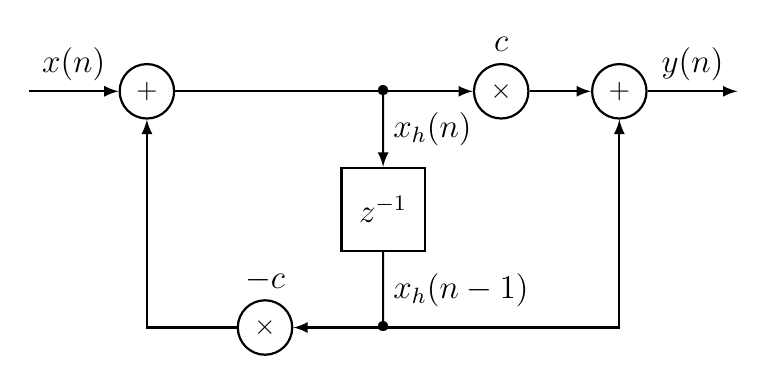
\begin{tikzpicture}[auto, thick, node distance=0.6cm, >=latex, scale = 0.75]
		\draw
		% Drawing the blocks of first filter 
		node at (0,0)[sum] (s1) {$+$}
		node at (6,0)[prod] (p1) {\product} node[above of = p1] {\large$c$}
		node at (8,0)[sum] (s2) {$+$}
		node at (4,-2) [delay] (d1) {\delay}
		node at (2,-4) [prod] (p2) {\product} node[above of = p2] {\large$-c$};
		
		\draw[->](-2,0) -- node {\large$x(n)$}(s1);
		\draw[->](s1) -- node {} (p1);
		\draw[->](p1) -- node {} (s2);
		\draw[->](s2) -- node {\large$y(n)$} (10,0);
		\draw[->](4,0) -- node {\large$x_h(n)$} (d1);
		\draw[->](p2) -| node {} (s1);
		\draw[-](d1) -- node {\large$x_h(n-1)$} (4,-4);
		\draw[<->](p2) -| node {} (s2);
		
		\draw
		node at (4,0) {\textbullet} 
		node at (4,-4){\textbullet};
		
		\end{tikzpicture}
	\end{center}
\end{frame}
\begin{frame}[fragile]
Corresponding state and output equations are:

\[
x_h(n) = -cx_h(n-1) +x(n)
\]
\[
y(n) = (1-c^2)x_h(n-1) + cx(n).
\]
Matlab code:
\begin{lstlisting}
function y = firstallpassunit(audio, para)
% y = firstallpass(audio, para)
% Author: Yangang Cao
% Applies a allpass filter to the input signal.
% para is the normalized cut-off frequency in (0,1)
c = (tan(pi*para/2)-1) / (tan(pi*para/2)+1);
x = 0;
x_1 = 0;
for n = 1:length(audio)
    x_1 = -c * x + audio(n);
    y(n) = (1 - c^2) * x + c * audio(n);
    x = x_1;
end
\end{lstlisting}

\end{frame}

\section{First-Order Low/Highpass Filter}


\frame{\frametitle{Outline}\tableofcontents[currentsection]}

\begin{frame}
\frametitle{First-Order Low/Highpass Filter}
A first-order lowpass/highpass filter can be achieved by adding or subtracting (+/--) the output signal from the input signal of a first-order allpass filter:
\[
H(z) = \frac{1}{2}(1 \pm A(z))\quad(LP/HP+/-)
\]
\[
A(z) = \frac{z^{-1} + c}{1 + cz^{-1}}
\]
\[
c = \frac{\tan(\pi f_c/f_S) - 1}{\tan(\pi f_c/f_S) + 1}.
\]
\end{frame}

\begin{frame}
Block diagram of first-order low/highpass filter 
\begin{center}
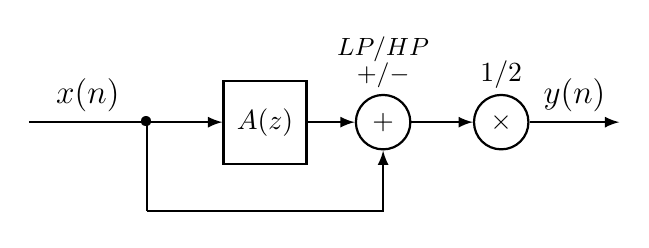
\begin{tikzpicture}[auto, thick, node distance=0.6cm, >=latex, scale = 0.75]
\draw
node at (2,0)[delay] (d1) {$A(z)$}
node at (4,0)[sum] (s1) {$+$} 
node[above of = s1]{\small$+/-$} node[above of=s1,above=1]{\small{$LP/HP$}}
node at (6,0) [prod] (p1) {\product} node[above of = p1]{$1/2$};

\draw[-](-2,0) -- node {\large$x(n)$}(0,0);
\draw[->](0,0) -- node {} (d1);
\draw[->](d1) -- node {} (s1);
\draw[->](s1) -- node {} (p1);
\draw[->](p1) -- node {\large$y(n)$} (8,0);
\draw[-](0,0) -- node {} (0,-1.5);
\draw[->](0,-1.5) -| node {} (s1);

\draw
node at (0,0) {\textbullet};

\end{tikzpicture}
\end{center}
\end{frame}
\subsection{first-order lowpass filter}
\begin{frame}
The difference equations of first-order lowpass filter are:
\[
x_h(n) = x(n) - cx_h(n-1)
\]
\[
y(n) = \frac{1+c}{2}x_h(n) + \frac{1+c}{2}x_h(n-1),
\]
and corresponding state and output equations are:
\[
x_h(n) = -cx_h(n-1) +x(n)
\]
\[
y(n) = \frac{1-c^2}{2}x_h(n-1) + \frac{1+c}{2}x(n).
\]
\end{frame}
\begin{frame}[fragile]
Matlab code:
\begin{lstlisting}
function y = aplowpassunit(audio, para)
% y = aplowpass(audio, para)
% Author: Yangang Cao
% Applies a lowpass filter to the input signal.
% para is the normalized cut-off frequency in (0,1)
c = (tan(pi*para/2)-1) / (tan(pi*para/2)+1);
x = 0;
x_1 = 0;
for n = 1:length(audio)
    x_1 = -c * x + audio(n);
    y(n) = ((1-c^2)/2) * x + (1+c)/2 * audio(n);
    x = x_1;   
end
\end{lstlisting}
\end{frame}
\subsection{first-order highpass filter}
\begin{frame}
The difference equations of first-order highpass filter are: 
\[
x_h(n) = x(n) - cx_h(n-1)
\]
\[
y(n) = \frac{1-c}{2}x_h(n) + \frac{c-1}{2}x_h(n-1)
\]
and corresponding state and output equations are:
\[
x_h(n) = -cx_h(n-1) +x(n)
\]
\[
y(n) = \frac{c^2-1}{2}x_h(n-1) + \frac{1-c}{2}x(n)
\]
\end{frame}
\begin{frame}[fragile]
Matlab code:
\begin{lstlisting}
function y = aphighpassunit(audio, para)
% y = aphighpass(audio, para)
% Author: Yangang Cao
% Applies a highpass filter to the input signal.
% para is the normalized cut-off frequency in (0,1)
c = (tan(pi*para/2)-1) / (tan(pi*para/2)+1);
x = 0;
x_1 = 0;
for n = 1:length(audio)
    x_1 = -c * x + audio(n);
    y(n) = ((c^2-1)/2) * x + (1-c)/2 * audio(n);
    x = x_1;  
end
\end{lstlisting}
\end{frame}
\end{document}